\documentclass{article}

\usepackage{amsmath}
\usepackage{amsfonts} % For math fonts.
\usepackage{amssymb} % For other math symbols not covered by amsmath.
\usepackage[pdftex]{graphicx} % For pictures, use \includegraphics[scale=decimal]{pic.png}; must be a .png file type.
\usepackage{multicol}
\usepackage{textcomp}
\usepackage[colorlinks = true, urlcolor = blue]{hyperref}
\usepackage{enumitem}
\usepackage{graphbox} 
\usepackage{subfig}
\usepackage{multicol}
\usepackage{nopageno}
\usepackage{bm}


\usepackage{tikz}
\usetikzlibrary{positioning, calc}
\usetikzlibrary{shapes.geometric,angles,quotes}
\usepackage{tikz-3dplot}


%page formatting
\usepackage{fullpage}
\setlength{\parindent}{0pt}


\newcommand{\tab}{\hspace*{0.25in}}
\newcommand{\csq}[1]{\reflectbox{''}#1''}  %This produces CS style quotes.
\newcommand{\csqt}[1]{\text{\reflectbox{''}#1''}}  %This produces CS style quotes as text.


\usepackage{listings}
\lstset
{ %Formatting for code in appendix
    language=Python,
    basicstyle=\footnotesize,
    numbers=left,
    stepnumber=1,
    showstringspaces=false,
    tabsize=2,
    breaklines=true,
    breakatwhitespace=false,
}


\begin{document}



%split_point

%\end{document}
Lone Star \hfill final retake quiz\\
section 4\\
\begin{enumerate}
\item (8.2) 	
		%https://edabit.com/challenge/yL5WmWTCNwwb4GnR7
		In each input list, every number repeats at least once, except for two. Write a \textbf{function} that takes an array $numbers$
		 and returns the two unique numbers.

		\textbf{Examples:}		
		\begin{itemize}
			\item  return\_unique([1, 9, 8, 8, 7, 6, 1, 6]) $\rightarrow$ [9, 7],
			\item  return\_unique([5, 5, 2, 4, 4, 4, 9, 9, 9, 1]) $\rightarrow$ [2, 1],
			\item  return\_unique([9, 5, 6, 8, 7, 7, 1, 1, 1, 1, 1, 9, 8]) $\rightarrow$ [5, 6]
		\end{itemize}




\item (8.3)
	Write a \textbf{function} that takes a dictionary, called $employee\_salaries$, where the keys are employee names and the values are their salaries. 
	The function should return a list of employees earning above a given salary.
	
	\textbf{Examples:}  
	\begin{itemize}  
		\item high\_earners(\{\csq{Alice}: 50000, \csq{Bob}: 75000, \csq{Charlie}: 100000\}, 60000) $\rightarrow$ [\csq{Bob}, \csq{Charlie}]
		\item high\_earners(\{\csq{David}: 30000, \csq{Emma}: 45000, \csq{Frank}: 50000\}, 40000) $\rightarrow$ [\csq{Emma}, \csq{Frank}]
		\item high\_earners(\{\csq{George}: 25000, \csq{Hannah}: 27000, \csq{Ian}: 29000\}, 30000) $\rightarrow$ []
	\end{itemize}


%end_of_questions
\item (13.3) % give playlist default name.
		Write a class for a \textbf{Playlist} with the instance variables and methods listed 
		below.\\
		A Playlist should have a default name of \csq{New Playlist}.\\
		It can be instantiated with initial songs, but it is not required to.\\
		Create a method called \textit{add\_song} which adds a song title (a string) to the 
		Playlist.\\
		You should be able to combine two Playlists, and print them in a readable way.
			
		\begin{minipage}[t]{0.65\textwidth}
			For example:
			\begin{itemize}
				\item $p_1 = [\csqt{Song A}, \csqt{Song B}]$
				\item $p_2 = [\csqt{Song C}]$
				\item $p_1 + p_2 = [\csqt{Song A}, \csqt{Song B}, \csqt{Song C}]$
			\end{itemize}

			Your class should support:
			\begin{itemize}
				\item Creating a playlist with a name and list of songs
				\item Adding two playlists (combines song lists)
				\item Printing the playlist in a readable way (e.g., list songs)
			\end{itemize}	
		\end{minipage}
		\hfill
		\begin{minipage}[t]{0.32\textwidth}
			\vspace{.2em}
			\begin{flushright}
				\begin{tabular}{|l|}
					\hline
					Playlist \\ \hline
					name \\
					songs (list of strings) \\ \hline
					\_\_init\_\_ \\
					add\_song \\
					\_\_add\_\_ \\
					\_\_str\_\_ \\ \hline
				\end{tabular}
			\end{flushright}
		\end{minipage}
		
		Once you have created the class, add code that:
		\begin{itemize}
			\item Creates two playlists and at least one song to each.
			\item Combines the playlists
			\item Prints the result
		\end{itemize}



\item (6.1) 
		%https://edabit.com/challenge/dBqLSk6qvudNdZrSx
		The \textbf{boiling point} of water is 212F in Fahrenheit and 100C in Celsuis. 
		Create a function that determines if the \textit{temp} is considered boiling or not.
		\textit{temp} will be measured in Fahrenheit and Celsuis.\\
		Notice: The F or C will always be the last character in the string.

	\textbf{Examples:}
	\begin{itemize}
		\item is\_boiling(\csq{212F}) $\rightarrow$ True, 
		\item is\_boiling(\csq{100C}) $\rightarrow$ True, 
		\item is\_boiling(\csq{0F}) $\rightarrow$ False, 
	\end{itemize}


\item (9.1) 
		(Game: Odd or Even)  Write a \textbf{function} that lets the user guess whether a randomly 
		generated number is odd or even.  The function randomly generates an integer between 0 and 9 
		(inclusive) and returns whether the user's guess is correct or incorrect. The argument for 
		the function will be $guess$ (the user's guess, either \csq{odd} or \csq{even}), if no 
		argument is provided then the \textbf{default} guess should be even.\\
		Hint: Use the following lines of code to create the function.
		\begin{verbatim}
		    from random import randint
		    value = randint(0,9) #picks a random integer between 0-9 inclusive
		\end{verbatim}
		\textbf{Examples:}
		\begin{itemize}
			\item  guess( ) $\rightarrow$ \csq{Correct!} (if random value is even) 
				or \csq{Incorrect!} (if random value is odd) 
			\item  guess(\csq{odd})$\rightarrow$\csq{Correct!} (if random value is odd) 
				or \csq{Incorrect!} (if random value is even)
			\item  guess(\csq{even}) $\rightarrow$ \csq{Correct!} (if random value is even) 
				or \csq{Incorrect!} (if random value is odd) 
		\end{itemize}


\end{enumerate}
\pagebreak
Dot Matrix \hfill final retake quiz\\
section 5\\
\begin{enumerate}
\item (4.1)  
		%https://edabit.com/challenge/Ay9wPrqRJnBmvbFmi
		Ask the user for two integers named \textit{larger} and \textit{smaller}.  
		Determine (and output) how many times larger can be halved while still be 
		greater than smaller.
		
		Examples:
		\begin{itemize}
			\item if \textit{larger} = 1324 and  \textit{smaller} = 98, the result should be 3 since
				1324 $\rightarrow$ 662 $\rightarrow$ 331 $\rightarrow$ 165.5
			\item if \textit{larger} = 624 and  \textit{smaller} = 8, the result should be 6 since\\
				\tab 624 $\rightarrow$ 312 $\rightarrow$ 156 $\rightarrow$ 78 $\rightarrow$ 39 
				$\rightarrow$ 19.5 $\rightarrow$ 9.75)
		\end{itemize}


\item (15.1) 
		Write a \textbf{program} that asks the user to enter the name of a text file and then prints 
		the contents of that file to the screen. The program should handle the following error:
		\begin{itemize}
			\item If the file does not exist (\textbf{FileExistsError}), print \csq{File not found.}
		\end{itemize}

		\textbf{Examples:}\\
			\begin{center}
			\includegraphics[scale=.65]{imgs/FileDirectoryExample.PNG}
			\end{center}
		\begin{itemize}
			\item \csq{Enter file name:} \csq{LunchData.txt} $\rightarrow$ 
				(prints the content of LunchData.txt)
			\item \csq{Enter file name:} \csq{DinnerData.txt} $\rightarrow$ \csq{File not found.}
		\end{itemize}
%Errors: FileNotFoundError


%end_of_questions

\item (3.1)  
		Write a program that asks the user for three numbers, and then determines (and outputs) 
		which of the numbers is the largest.  Do not use the built-in function \textit{max}().\\
		For example, \\ \ \hfill
		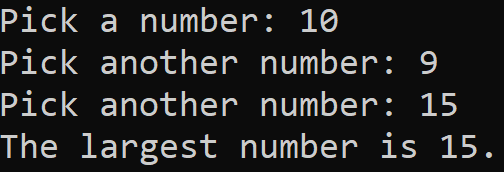
\includegraphics[height = 0.6in]{./imgs/largest_ex1.PNG} \hfill
		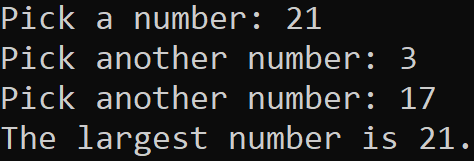
\includegraphics[height = 0.6in]{./imgs/largest_ex2.PNG} \hfill \ 



\item (15.2) 
		You are helping a teacher update students' scores after a quiz.  
		The teacher wants to add points for extra credit and needs your program to 
		do the math safely.\\

		A dictionary stores the number of points each student has earned, shown below: 
		\begin{itemize}
			\item \texttt{\{\csq{Alice}: 90, \csq{Bob}: 75, \csq{Charlie}: 60\}}
		\end{itemize}
		Write a \textbf{program} that asks the user to enter a student's name and a number 
		to add to their score. The program should print the new number of points.

		The program should handle the following errors:
		\begin{itemize}
			\item If the name is not found in the dictionary (\textbf{KeyError}), 
				print \csq{Student not found.}
			\item If the number entered is not valid (e.g., not a number) (\textbf{ValueError}), 
				print \csq{Invalid number.}
		\end{itemize}

		\textbf{Examples:}
		\begin{itemize}
			\item \csq{Enter student name:} \csq{Bob} \\
			      \csq{Enter number to add:} 10 $\rightarrow$ 85
			\item \csq{Enter student name:} \csq{David} $\rightarrow$ \csq{Student not found.}
			\item \csq{Enter student name:} \csq{Alice} \\
			      \csq{Enter number to add:} \csq{ten} $\rightarrow$ \csq{Invalid number.}
		\end{itemize}

%Errors: KeyError, ValueError




%%%%%%%%%%%%%%%%%%%%%
	% Problem 6
	% Difficulty: 2
%%%%%%%%%%%%%%%%%%%%%
\item (3.2)  
		Write a program that prompts the user to enter three integers and displays the integers 
		in decreasing order (largest to smallest).  You may not use the built-in functions 
		\textit{max}(), \textit{min}(), \textit{sort}() or \textit{sorted}().



\end{enumerate}
\pagebreak
Dark Helmet \hfill final retake quiz\\
section 4\\
\begin{enumerate}
\item (4.2)   
		Write a program to create a word one letter at a time.  You should prompt the user to enter 
		a single letter one at a time until they type \textit{done}.  Once they type done, output 
		their newly created word.
		
		For example, \\ \ \hfill
		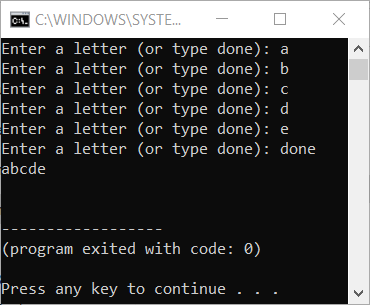
\includegraphics[width = 2.5in]{./imgs/lettersAbcde.PNG} \hfill  
		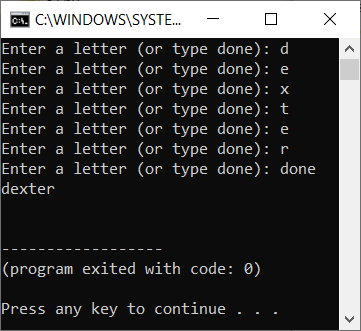
\includegraphics[width = 2.5in]{./imgs/lettersDexter.PNG} \hfill \


\item (15.3) 
		You've been asked to help build part of a travel booking system.  
		One of the features lets users type in a country code (like \csq{US}) and shows them the 
		full country name to confirm their destination.

		A dictionary stores some country codes, shown below: 
			$$\texttt{\{\csq{US}:\csq{United States}, \csq{FR}:\csq{France}, 
				\csq{JP}:\csq{Japan}, \csq{BR}:\csq{Brazil}\}}$$
		Write a \textbf{program} that asks the user to enter a country code (like \csq{US}) 
		and then prints the full country name. If the user enters an invalid code, they should 
		be asked to try again until a valid code is entered.

		The program should handle the following errors:
		\begin{itemize}
			%\item If the input is empty, print \csq{Invalid input. Try again.}
			\item If the code is not found in the dictionary (\textbf{KeyError}), 
				print \csq{Code not found. Try again.}
		\end{itemize}

		\textbf{Examples:}
		\begin{itemize}
			\item \csq{Enter a country code:} \csq{JP} $\rightarrow$ \csq{Japan}
			\item \csq{Enter a country code:} \csq{XYZ} $\rightarrow$ 
				\csq{Code not found. Try again.}
			%\item \csq{Enter a country code:} \csq{} $\rightarrow$ \csq{Invalid input. Try again.}
			\item (after retry) \csq{Enter a country code:} \csq{BR} $\rightarrow$ \csq{Brazil}
		\end{itemize}

%Errors: KeyError, ValueError


%%%%%%%%%%%%%%%%%%%%%
	% Problem 10
	% Difficulty: 3
%%%%%%%%%%%%%%%%%%%%%
\item (2.1)
		%https://edabit.com/challenge/QzXtDnSZL6y4ZcEvT
		A farmer is asking you to tell him how many legs can be counted among all his animals. 
		The farmer breeds three species:
		\begin{itemize}
			\item chickens, which have \textbf{2} legs
			\item cows, which have \textbf{4} legs
			\item pigs, which have \textbf{4} legs
		\end{itemize}
		Write a program that asks the farmer how many of each animal he has, and then outputs the
		total number of legs.  		
		For example, \\ \ \hfill
		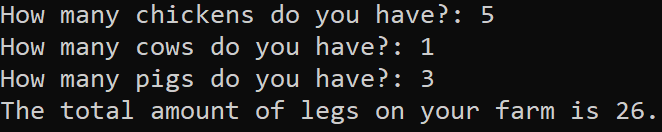
\includegraphics[height = 0.6in]{./imgs/animalLegs_ex1.PNG} \hfill
		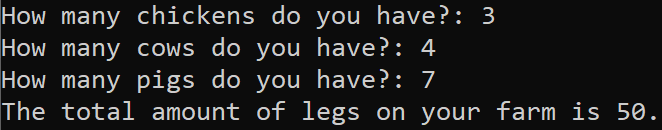
\includegraphics[height = 0.6in]{./imgs/animalLegs_ex2.PNG} \hfill \


\item (15.1) 
		Write a \textbf{program} that asks the user to enter the name of a text file and then prints 
		the contents of that file to the screen. The program should handle the following error:
		\begin{itemize}
			\item If the file does not exist (\textbf{FileExistsError}), print \csq{File not found.}
		\end{itemize}

		\textbf{Examples:}\\
			\begin{center}
			\includegraphics[scale=.65]{imgs/FileDirectoryExample.PNG}
			\end{center}
		\begin{itemize}
			\item \csq{Enter file name:} \csq{LunchData.txt} $\rightarrow$ 
				(prints the content of LunchData.txt)
			\item \csq{Enter file name:} \csq{DinnerData.txt} $\rightarrow$ \csq{File not found.}
		\end{itemize}
%Errors: FileNotFoundError


%end_of_questions

\item (15.2) 
		You are helping a teacher update students' scores after a quiz.  
		The teacher wants to add points for extra credit and needs your program to 
		do the math safely.\\

		A dictionary stores the number of points each student has earned, shown below: 
		\begin{itemize}
			\item \texttt{\{\csq{Alice}: 90, \csq{Bob}: 75, \csq{Charlie}: 60\}}
		\end{itemize}
		Write a \textbf{program} that asks the user to enter a student's name and a number 
		to add to their score. The program should print the new number of points.

		The program should handle the following errors:
		\begin{itemize}
			\item If the name is not found in the dictionary (\textbf{KeyError}), 
				print \csq{Student not found.}
			\item If the number entered is not valid (e.g., not a number) (\textbf{ValueError}), 
				print \csq{Invalid number.}
		\end{itemize}

		\textbf{Examples:}
		\begin{itemize}
			\item \csq{Enter student name:} \csq{Bob} \\
			      \csq{Enter number to add:} 10 $\rightarrow$ 85
			\item \csq{Enter student name:} \csq{David} $\rightarrow$ \csq{Student not found.}
			\item \csq{Enter student name:} \csq{Alice} \\
			      \csq{Enter number to add:} \csq{ten} $\rightarrow$ \csq{Invalid number.}
		\end{itemize}

%Errors: KeyError, ValueError




%%%%%%%%%%%%%%%%%%%%%
	% Problem 6
	% Difficulty: 2
%%%%%%%%%%%%%%%%%%%%%

\end{enumerate}
\pagebreak
President Skroob \hfill final retake quiz\\
section 1\\
\begin{enumerate}
\item (15.3) 
		You've been asked to help build part of a travel booking system.  
		One of the features lets users type in a country code (like \csq{US}) and shows them the 
		full country name to confirm their destination.

		A dictionary stores some country codes, shown below: 
			$$\texttt{\{\csq{US}:\csq{United States}, \csq{FR}:\csq{France}, 
				\csq{JP}:\csq{Japan}, \csq{BR}:\csq{Brazil}\}}$$
		Write a \textbf{program} that asks the user to enter a country code (like \csq{US}) 
		and then prints the full country name. If the user enters an invalid code, they should 
		be asked to try again until a valid code is entered.

		The program should handle the following errors:
		\begin{itemize}
			%\item If the input is empty, print \csq{Invalid input. Try again.}
			\item If the code is not found in the dictionary (\textbf{KeyError}), 
				print \csq{Code not found. Try again.}
		\end{itemize}

		\textbf{Examples:}
		\begin{itemize}
			\item \csq{Enter a country code:} \csq{JP} $\rightarrow$ \csq{Japan}
			\item \csq{Enter a country code:} \csq{XYZ} $\rightarrow$ 
				\csq{Code not found. Try again.}
			%\item \csq{Enter a country code:} \csq{} $\rightarrow$ \csq{Invalid input. Try again.}
			\item (after retry) \csq{Enter a country code:} \csq{BR} $\rightarrow$ \csq{Brazil}
		\end{itemize}

%Errors: KeyError, ValueError


%%%%%%%%%%%%%%%%%%%%%
	% Problem 10
	% Difficulty: 3
%%%%%%%%%%%%%%%%%%%%%
\item (2.3)
		Write a program that calculates the volume of a cylinder.  The user should be able to pick
		the height and radius.  Use the value of $\pi$ from the math module in your calculation.\\
		\tab Hint: $V = \pi r^2 h$\\

		\vspace*{-2em}
		\begin{flushright}
		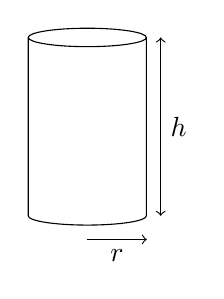
\begin{tikzpicture}
			\node (a) [cylinder, shape border rotate=90, draw, 
				minimum height=25mm, minimum width=15mm] {};
			\draw [<->] ([xshift=5pt]a.before bottom) -- ([xshift=5pt]a.after top)
				 node [midway, right] {$h$};
			\draw [->] ([yshift=-5pt]a.bottom) -- ([yshift=-5pt]a.bottom -| a.before bottom)
				node [midway, below] {$r$};
		\end{tikzpicture}
		\end{flushright}


\item (4.2)  
		Write a program that repeatedly asks the user for integers until a negative integer is 
		given. \\ The program should keep track of the sum of the numbers and print the sum at the 
		end \\(not including the negative number).

		For example, \\ \ \hfill
		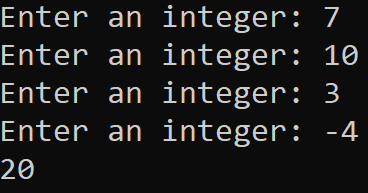
\includegraphics[width = 2.in]{./imgs/AddCalc2.PNG} \hfill  
		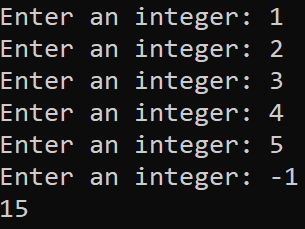
\includegraphics[width = 2.in]{./imgs/AddCalc1.PNG} \hfill \


\item (4.3)  
		%https://edabit.com/challenge/xR248CxGSsSrNK5Za
		You are the newest rug fashion designer on the scene, but you're running out of ideas. 
		Write a program that will help you design rugs.  The program should ask for a width, 
		a length, and pattern, and then create a rug consisting of that pattern and dimensions.

		For example, \\ \ \hfill
		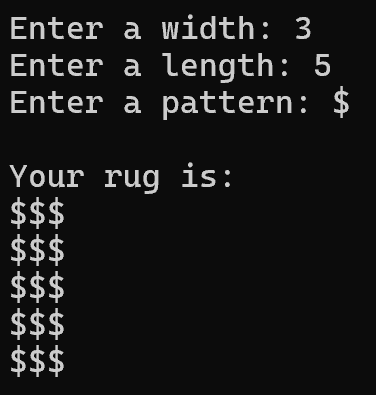
\includegraphics[width = 1.5in]{./imgs/rug1.PNG} \hfill  
		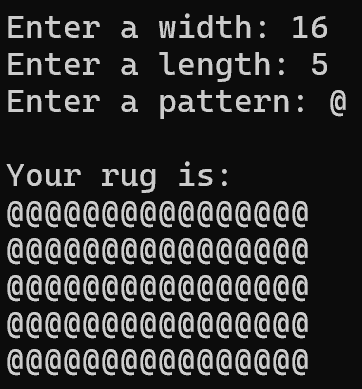
\includegraphics[width = 1.5in]{./imgs/rug2.PNG} \hfill \


\item (2.2) 
		Write a program that calculates then outputs the volume of a right square pyramid.  
		The user should be able to pick $b$ (the base edge) and $h$ (the height).\\
		%Make sure to use the value of pi from the math module.\\
		Hint: $V = \dfrac{b^2 h}{3}$
		
		\vspace*{-4em}
		\begin{flushright}
		\tdplotsetmaincoords{70}{-20}
		\begin{tikzpicture}[tdplot_main_coords,line cap=butt,line join=bevel]
			\pgfmathsetmacro{\B}{4}
			\pgfmathsetmacro{\H}{4}
			\draw[thick] (-\B/2,-\B/2,0) -- (\B/2,-\B/2,0) -- (\B/2,\B/2,0) -- (-\B/2,\B/2,0)
				 -- cycle;
			\draw[thick] (\B/2,\B/2,0) -- (0,0,\H)
			node[above,font=\large\bfseries]{};
			\draw[dashed] (0,0,0) -- (0,0,\H) coordinate[midway](aux1);
			\draw[] (0,0,0.3) -- (0.3,0,0.3) -- (0.3,0,0);
			%\draw[dashed,blue] (-\B/2,0,0) -- (0,0,\H) coordinate[pos=0.3](aux2);
			%\draw[blue] ({-\B/2+0.15*(\H/\B)},0,0.3) -- ({-\B/2+0.15*(\H/\B)},-0.3,0.3) 
				%-- (-\B/2,-0.3,0);
			\coordinate (aux3) at (0.3,-2,0);
			\draw[thick] (-\B/2,-\B/2,0) -- (0,0,\H) -- (\B/2,-\B/2,0) -- cycle;
			\draw[thick] (-\B/2,-\B/2,0) -- (0,0,\H) -- (-\B/2,\B/2,0) -- cycle;
			\begin{scope}[tdplot_screen_coords]
				\draw (aux1) -- ++ (2,0.1) node[right,font=\itshape] {Height: h};
				%\draw (aux2) -- ++ (-1.5,0.3) node[left,font=\itshape] {Slant Height};
				\draw (aux3) -- ++ (2,-0.2) node[below right,font=\itshape] {Base edge: b};
			\end{scope}
		\end{tikzpicture}
		\end{flushright}

%end_of_questions

\end{enumerate}
\pagebreak
\end{document}